\documentclass[12pt]{article}

\usepackage[utf8]{inputenc}
\usepackage[english, russian]{babel}

\usepackage{slides}

\hyphenpenalty=5000
\tolerance=1000

% ШРИФТЫ
% Нужны рубленные шрифты -- раскомментируйте стоку ниже. 
% Нужны шрифты с засечками --- закомментируйте эту строку. 
\renewcommand{\familydefault}{\sfdefault} % Переключает на рубленный шрифт.
% Шрифты Times и Arial, если стоит пакет cyrtimes. 
% Если он не стоит, результат будет плохой!
%\usepackage{cyrtimespatched}
% Если нет cyrtimes, то попробуйте включить полужирный шрифт:
% \renewcommand{\seriesdefault}{b} % для шрифта с засечками, это предпочтительно
% \renewcommand{\seriesdefault}{sbc} % для рубленного шрифта

\usepackage{graphicx}
\usepackage{alltt}

\usepackage{listings}
% Значения по умолчанию для listings
\lstset{
  breakatwhitespace=true,% разрыв строк только на whitespacce
  breaklines=true,       % переносить длинные строки
  captionpos=b,          % подписи снизу
  extendedchars=\true,   % допуск utf
  inputencoding=utf8,
  numbers=left,          % нумерация слeва
  showspaces=false,      % показывать пробелы подчеркиваниями -- идиотизм 70-х годов
  showstringspaces=false,
  showtabs=false,        % и табы тоже
  stepnumber=1,
  tabsize=4              % кому нужны табы по 8 символов?..
}


% Стиль для псесдовода: строчки обычно короткие, поэтому размер шрифта побольше
\lstdefinestyle{pseudocode}{
  basicstyle=\small,
  frame=none,
  keywordstyle=\color{black}\bfseries\underbar,
  language=Pseudocode,
  numberstyle=\footnotesize
}

% Стиль для обычного кода: маленький шрифт
\lstdefinestyle{realcode}{
  basicstyle=\scriptsize,
  frame=none,
  numberstyle=\footnotesize
}

% Стиль для коротких кусков обычного кода: средний шрифт
\lstdefinestyle{simplecode}{
  basicstyle=\footnotesize,
  frame=none,
  numberstyle=\footnotesize
}

% Определим свой язык для написания псевдокодов на основе Python
\lstdefinelanguage[]{Pseudocode}[]{Python}{
  morekeywords={each,empty,wait,do},% ключевые слова добавлять сюда
  morecomment=[s]{\{}{\}},% комменты {а-ля Pascal} смотрятся нагляднее
  literate=% а сюда добавлять операторы, которые хотите отображать как мат. символы
    {->}{\ensuremath{$\rightarrow$}~}2%
    {<-}{\ensuremath{$\leftarrow$}~}2%
    {:=}{\ensuremath{$\leftarrow$}~}2%
}[keywords,comments]

\def\Student{Коротков Иван Андреевич}
\def\Advisor{Крищенко Всеволод Александрович}
\def\ShortTitle{Параллельное построение пространства состояний конечной модели для проверки ее свойств}
\def\Title{Параллельное построение пространства состояний конечной модели для проверки ее свойств}
\def\SubTitle{Квалификационная работа магистра}

% Верхний заголовок: пустой
% Нижний заголовок по-умолчанию:
\lfoot{\ShortTitle} % слева
% \cfoot{} % цент пуст
% \rfoot{\thepage} % справа

% \renewcommand{\baselinestretch}{1.5}
 \linespread{1.2}

%\hyphenpenalty=0

\begin{document}

\TitleSlide

\section{Классы ошибок в ПО и методы их устранения}
\label{sec:error-classes}

\begin{center}
  \begin{tabular}{|c|c|c|} \hline Вероятность & \multicolumn{2}{|c|}{Степень критичности}
    \\ \cline{2-3} возникновения & Высокая & Низкая \\ \hline
    Высокая & Тестирование & Тестирование \\ \hline Низкая & Проверка модели & \\
    \hline
  \end{tabular}
\end{center}

\section{Цель и задачи}
\label{sec:goal-tasks}

Разработка и исследование метода параллельной генерации состояний конечной
детерминированной модели.

\small
\begin{itemize}
\item Проанализировать проблемы проверки моделей и существующие подходы к их решению
\item Разработать и реализовать алгоритм параллельной генерации состояний
\item Спроектировать метод автоматического распределения состояний между узлами
\item Провести эксперименты и проанализировать их результаты
\end{itemize}
\normalsize

\section{Автомат Мили для задачи о философах}
\label{sec:mealey}

\begin{center}
  \includegraphics[height=0.85\textheight]{../graphics/philo-mealey}
\end{center}

\section{Модель Крипке: определение}
\label{sec:kripke-def}

Модель Крипке $M$ над множеством атомарных высказываний $A$~--- четверка $M=(S, S_0, R,
L)$, где:
\begin{enumerate}
\item $S$~--- конечное множество состояний;
\item $S_0 \subseteq S$~--- множество начальных состояний;
\item $R \subseteq S \times S$~--- тотальное отношение переходов: $$\forall s \in S\colon \exists
  s' \in S \colon R(s, s')$$
\item $L: S \rightarrow 2^{A}$~--- функция, которая помечает каждое состояние множеством
  атомарных высказываний, истинных в этом состоянии.
\end{enumerate}

\section{Модель Крипке для системы из двух философов}
\label{sec:kripke-philo}

\begin{center}
  \includegraphics[height=0.85\textheight]{../graphics/philo-kripke}
\end{center}

\section{Описание модели философов на языке Promela}
\label{sec:prml-philo}

\begin{lstlisting}[language=Promela,style=simplecode]
bit  fork[5]
byte nr_eat

active [5] proctype Philosopher() {
Think:
  atomic { fork[_pid] == 0 -> fork[_pid] = 1 };
One:
  atomic { fork[(_pid + 1)%5] == 0 -> fork[(_pid + 1)%5] = 1; 
           nr_eat++ };
Eat:
  atomic { nr_eat--; fork[(_pid + 1)%5] = 0 };
  fork[_pid] = 0;
  goto Think
}  
\end{lstlisting}

\section{Проверка конечных моделей}
\label{sec:verif-troubles}

\begin{itemize}
\item Размер пространства состояний растет экспоненциально

\item Модели среднего размера требуют более 10 Гб оперативной памяти для хранения
  пространства состояний
\end{itemize}

\begin{minipage}[t]{0.5\linewidth}
  \begin{flushleft}
    \begin{itemize}
    \item Использование битового \mbox{хэширования}
    \item Сжатие хранимых состояний
    \item Метод сокращение частных порядков
    \end{itemize}
  \end{flushleft}
\end{minipage}
\begin{minipage}[t]{0.5\linewidth}
  \begin{flushleft}
    \begin{itemize}
    \item Параллельная \mbox{генерация} состояний
    \end{itemize}
  \end{flushleft}
\end{minipage}

\section{Алгоритм распределенного хранения состояний}
\label{sec:distr-storage}

\begin{lstlisting}[style=pseudocode]
Visited = ()

def ParStateSpaceDFS(state):
    node = StateNode(state)
    if not state in node.Visited:
        node.Visited <- state
        for each new_state in Next(state):
            StateSpaceDFS(new_state)

ParStateSpaceDFS(initial_state)
\end{lstlisting}

\section{Пример работы алгоритма распределенного хранения}
\label{sec:distr-storage2}

\begin{minipage}[m]{0.5\linewidth}
  \includegraphics[height=0.85\textheight]{../graphics/distr-storage}
\end{minipage}
\begin{minipage}[m]{0.5\linewidth}
  \begin{flushleft}
    \begin{itemize}
    \item Используется вычислительная мощность лишь одного узла
    \item Большое число удаленных вызовов
    \item Удаленные вызовы синхронные
    \end{itemize}
  \end{flushleft}
\end{minipage}

\section{Алгоритм распределенной генерации состояний}
\label{sec:distr-generation}

\begin{lstlisting}[style=pseudocode]
Visited = ()
Queue   = (initial_state)
def ParStateSpaceBFS():
    while not empty(Queue):
        Queue -> state
        node = StateNode(state)
        if NodeId = node:
            if not state in Visited:
                Visited <- state
                for each new_state in Next(state):
                    Queue <- new_state
        else:
            node.Queue <- state
ParStateSpaceBFS()
\end{lstlisting}

\section{Пример работы алгоритма распределенной генерации}
\label{sec:distr-generation2}

\begin{minipage}[m]{0.55\linewidth}
  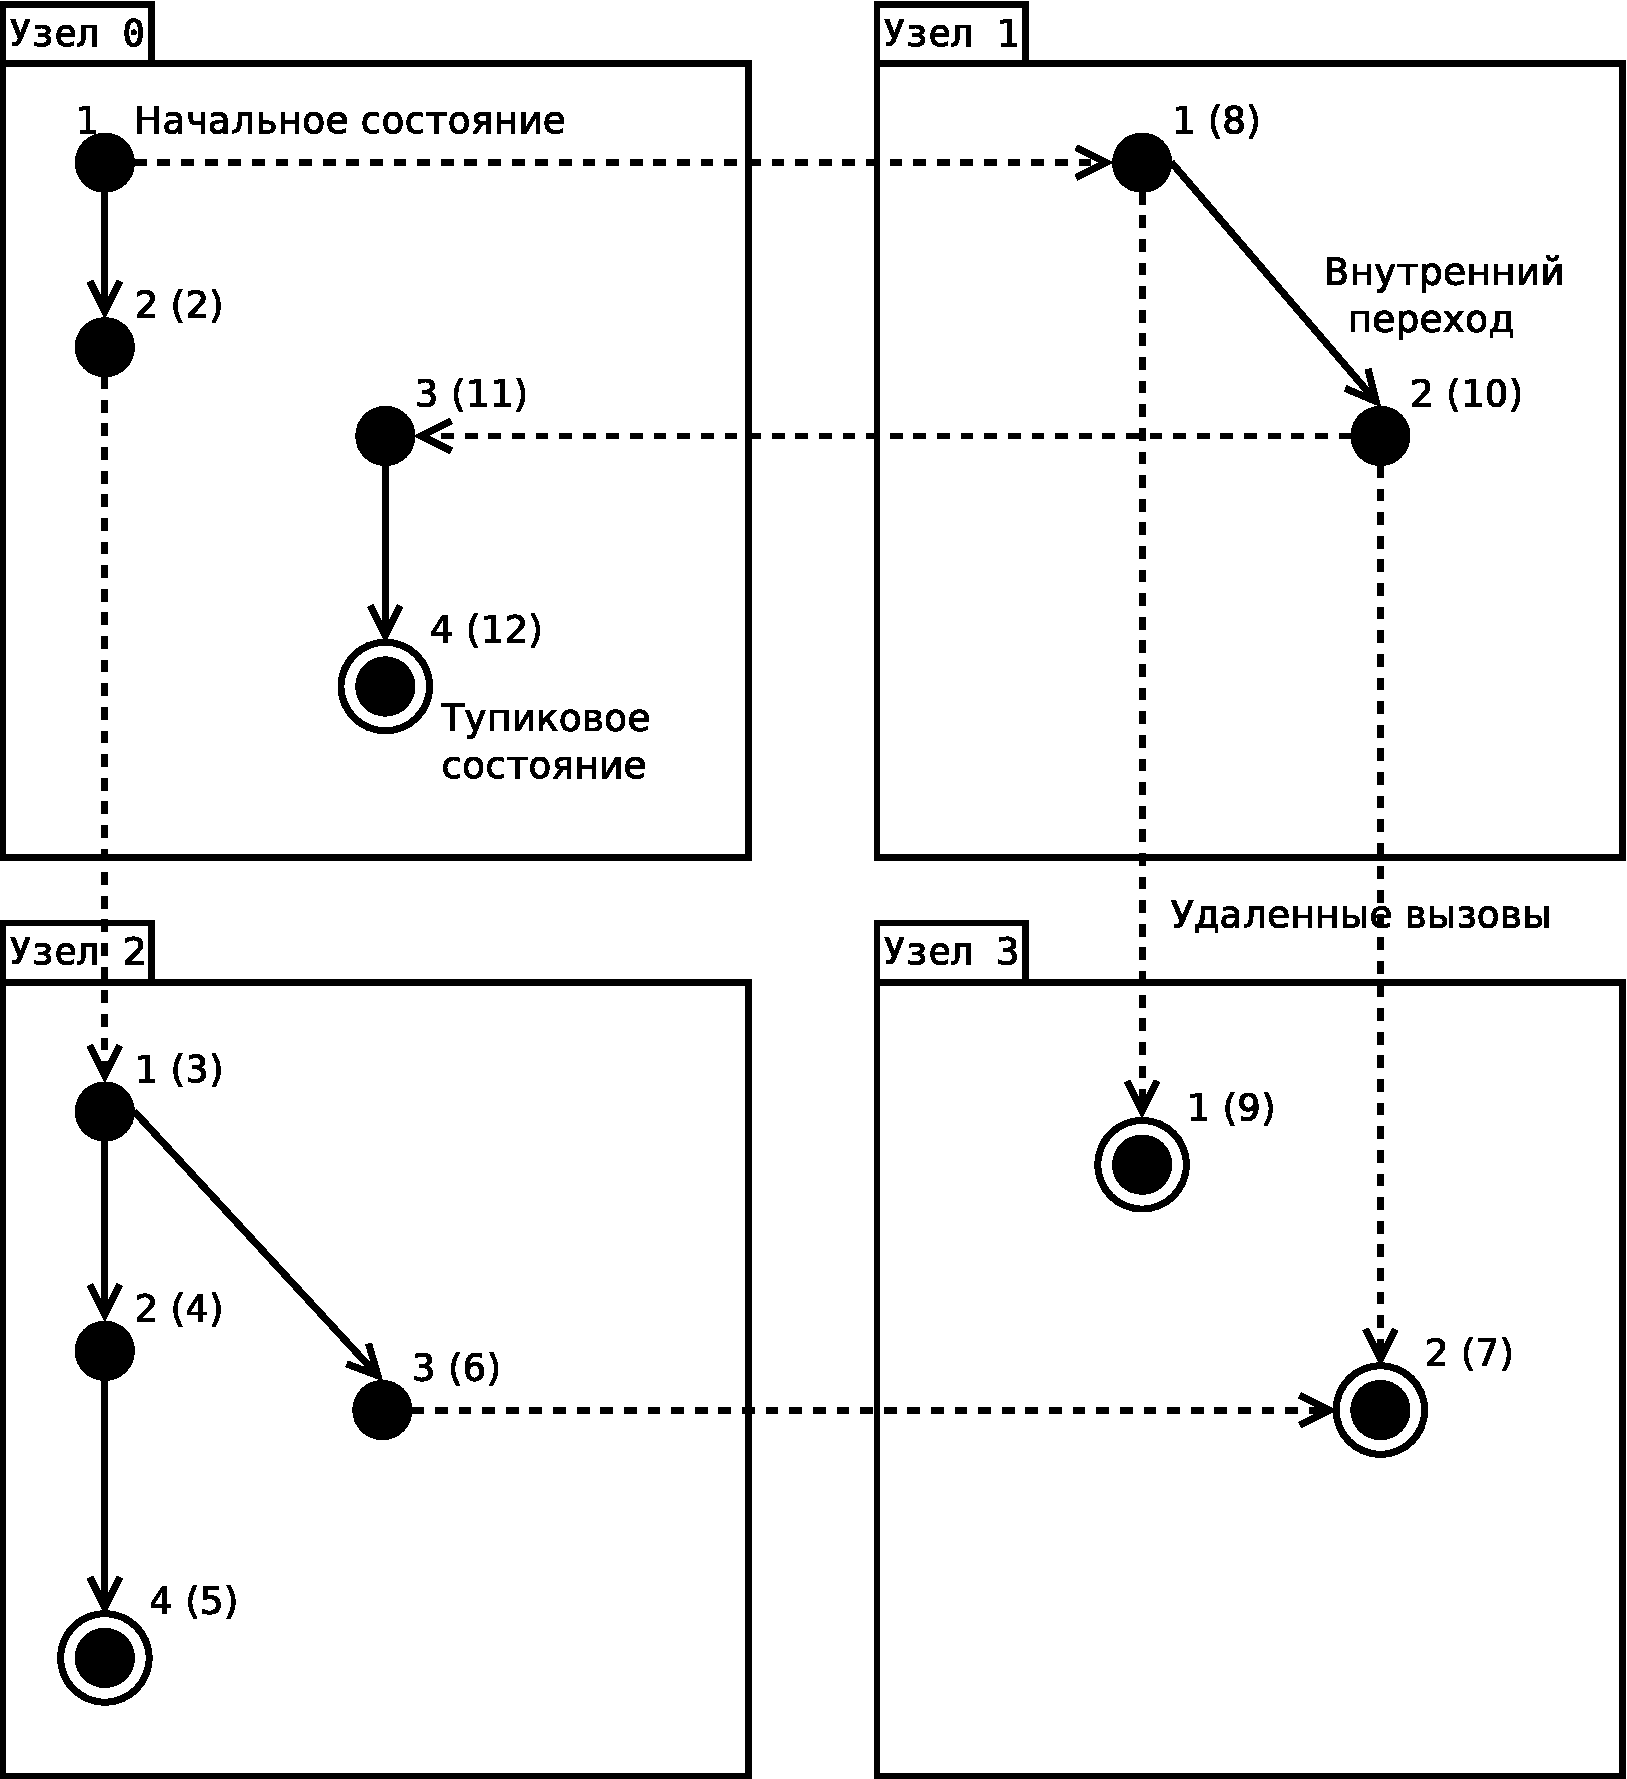
\includegraphics[height=0.85\textheight]{../graphics/distr-generation}
\end{minipage}
\begin{minipage}[m]{0.45\linewidth}
  \begin{flushleft}
    \begin{itemize}
    \item Используется вычислительная мощность всех узлов
    \item Удаленные вызовы асинхронные
    \item Можно уменьшить число удаленных вызовов
    \end{itemize}
  \end{flushleft}
\end{minipage}

\section{Распределение состояний между узлами}
\label{sec:state-partitioning}

\begin{center}
  \includegraphics[width=0.9\textwidth]{../graphics/state-partition}
\end{center}

\section{Хранение состояний в ОЗУ узла}
\label{sec:state-store-full}

\begin{center}
  \includegraphics[width=0.9\textwidth]{../graphics/fullstate}
\end{center}

\section{Компоненты параллельного генератора}
\label{sec:component-diag}

\begin{center}
  \includegraphics[height=0.88\textheight]{../graphics/components}
\end{center}

\section{Развертывание параллельного генератора}
\label{sec:deployment-diag}

\begin{center}
    \includegraphics[height=0.88\textheight]{../graphics/mpi-deploy}
\end{center}

\section{Алгооритм отправки сообщений удаленному узлу}
\label{sec:mpi-send-flowchart}

\begin{center}
  \includegraphics[height=0.88\textheight]{../graphics/mpi-send-flowchart-horz}
\end{center}

\section{Взаимодействие двух MPI-процессов}
\label{sec:mpi-sequence}

\begin{center}
  \includegraphics[height=0.88\textheight]{../graphics/mpi-async-seq}
\end{center}

\section{Трансляция описания модели в граф команд}
\label{sec:pmlparse}

\begin{minipage}[m]{0.35\linewidth}
  \begin{lstlisting}[language=Promela,style=simplecode,numbers=none]
    do
    :: x == 1 -> y = 2
    :: x == 2 -> y = 1
    :: else  -> break
    od;
    channel1 ! x,y
  \end{lstlisting}
\end{minipage}
\begin{minipage}[m]{0.75\linewidth}
  \includegraphics[height=0.85\textheight]{../graphics/pmlparse-inner}
\end{minipage}

\section{Содержание экспериментов}
\label{sec:experim}

\begin{itemize}
\item Сравнение разработанного ПО с существующим
\item Сравнение методов распределения состояний
\end{itemize}

\begin{center}
  \includegraphics[width=1\textwidth]{../graphics/exp-idef0}
\end{center}

\section{Зависимость требуемого времени от числа состояний}
\label{sec:states-time}

\begin{center}
  \includegraphics[height=0.88\textheight]{../data/plots/states-speed}
\end{center}

\section{Сравнение скорость генерации состояний}
\label{sec:stategen-speed}

\begin{tabular}{ccccc}
  \hline
  Модель & Число     & ПО Spin,   & Разработанное ПО, & Отношение \\
  & процессов & сост./сек &  сост./сек         & скоростей \\
  \hline
  Election & 6 & 1622583 & 2179986 & 1.3 \\
  Peterson & 4 & 3940962 & 2082656 & 0.5 \\
   & 5 & 2538418 & 2657356 & 1.0 \\
  Philo & 5 & 3063200 & 1223386 & 0.4 \\
   & 6 & 3080406 & 1893468 & 0.6 \\
  \hline
\end{tabular}

\section{Сравнение методов распределения состояний}
\label{sec:partition-cmp}

\begin{minipage}[m]{0.5\linewidth}
  \includegraphics[width=1.1\textwidth,page=1]{../data/plots/state-partition1-horz}  
\end{minipage}
\begin{minipage}[m]{0.5\linewidth}
  \includegraphics[width=1.1\textwidth,page=2]{../data/plots/state-partition1-horz}  
\end{minipage}

% Отношение числа MPI-сообщений к числу переходов между состояниями модули

\section{Выводы}
\label{sec:conclusion}

\small
\begin{enumerate}
\item Проанализированы проблемы проверки моделей и существующие подходы к их решению
\item Спроектирован и реализован алгоритм параллельной генерации состояний конечной
  модели
\item Предложен метод автоматического распределения состояний, уменьшающий число сообщений
  между узлами
\item Проведены эксперименты и проанализированы их результаты
\end{enumerate}

По результатам работы имеется одна публикация.

\end{document}

%%% Local Variables: 
%%% mode: latex
%%% TeX-master: t
%%% End: 
